	\frame
	{
		\frametitle{Store}
		Un objet (image, s\'erie, examen, rapport de dose, \ldots) cr\'e\'e par une modalit\'e d'imagerie peut \^etre stock\'ee sur un syst\^eme d'archivage DICOM comme un PACS ou une VNA pour peu qu'il respecte les exigences d'une \emph{Information Object Definition} (IOD).
		\begin{itemize}
			\item<2-> L'IOD d\'efinit les attributs qu'on doit ou peut trouver dans l'objet.
			\item<3-> DICOM divise une IOD en \emph{Information Entities} (IE). Cela permet de d\'efinir des blocs qui seront communs entre diff\'erents types de donn\'ees.
			\item<4-> Une IE est l'association d'un ou plusieurs \emph{Modules}, qui sont
			\begin{description}
				\item<5->[Mandatory] obligatoires,
				\item<6->[Conditional] conditionnels,
				\item<7->[User Option] ou optionnels.
			\end{description}
	   		\item<8-> Les modules indiquent quels attributs peuvent ou doivent \^etre pr\'esents dans l'object \`a stocker
			\begin{description}
				\item<9->[1] Obligatoire.
				\item<9->[2] Obligatoire~-~peut \^etre vide.
				\item<9->[3] Optionnel.
				\item<9->[<1/2>C] Conditionnel.
			\end{description}
		\end{itemize}
	}
	
	% \frame
	% {
 	% 	\frametitle{IOD composite}
	% 	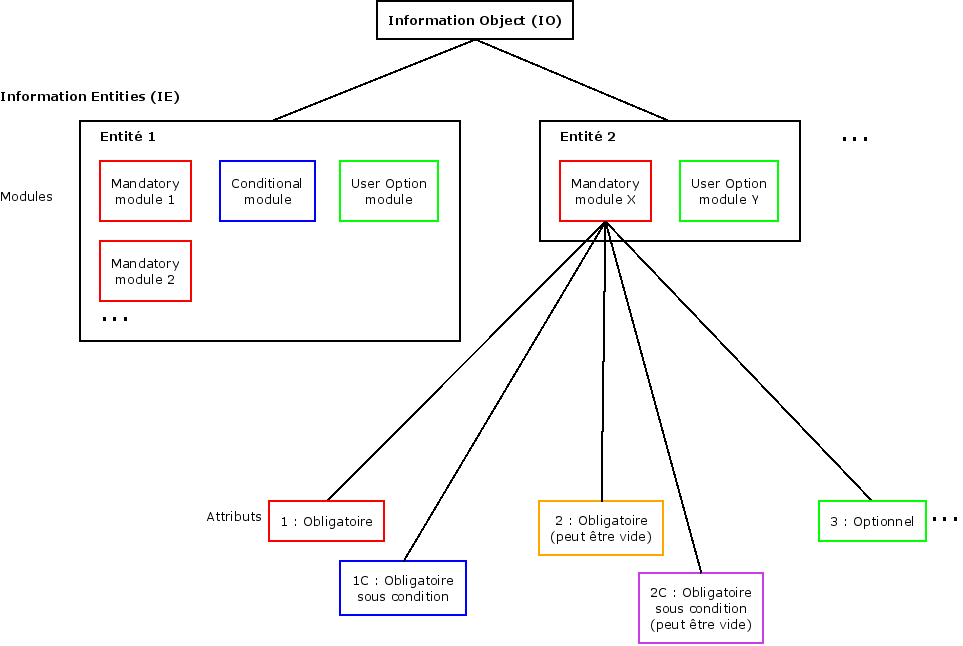
\includegraphics[width=\linewidth]{./figures/IO-composite.png}
	% }

	% \frame
	% {
	% 	\frametitle{Exemple d'IOD : DICOM SR}
	% 	\url{http://dicom.nema.org/medical/dicom/current/output/chtml/part03/sect_A.35.3.3.html}
	% 	\begin{center}
	% 		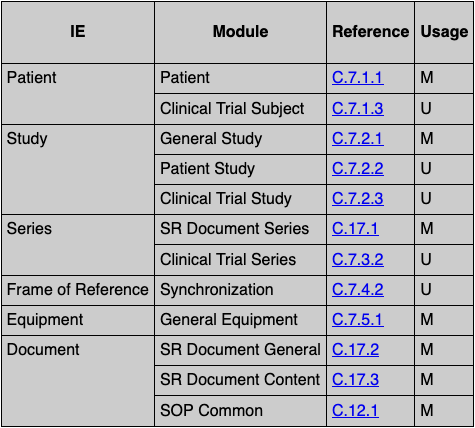
\includegraphics[width=0.5\linewidth]{./figures/IOD-exemple-SR.png}
	% 	\end{center}
	% }

	\frame
	{
		\frametitle{Exemple d'IOD: image CR}
		\url{http://dicom.nema.org/medical/dicom/current/output/chtml/part03/sect_A.2.3.html}
		\begin{center}
			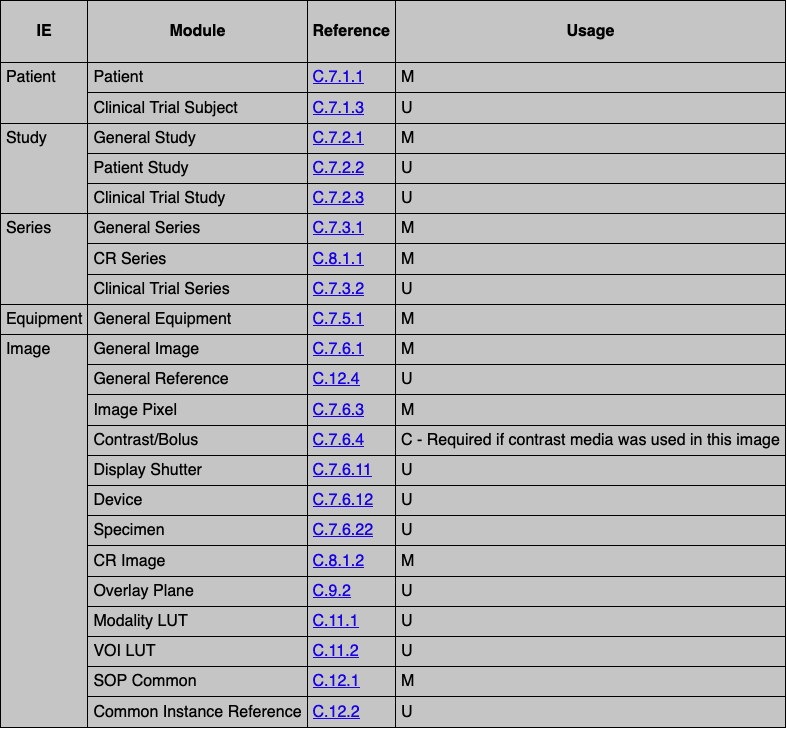
\includegraphics[width=0.6\linewidth]{../figures/IOD-exemple-CR.png}
		\end{center}
	}

	\frame
	{
		\frametitle{Sch\'ema de l'IOD image CR}
		\begin{center}
			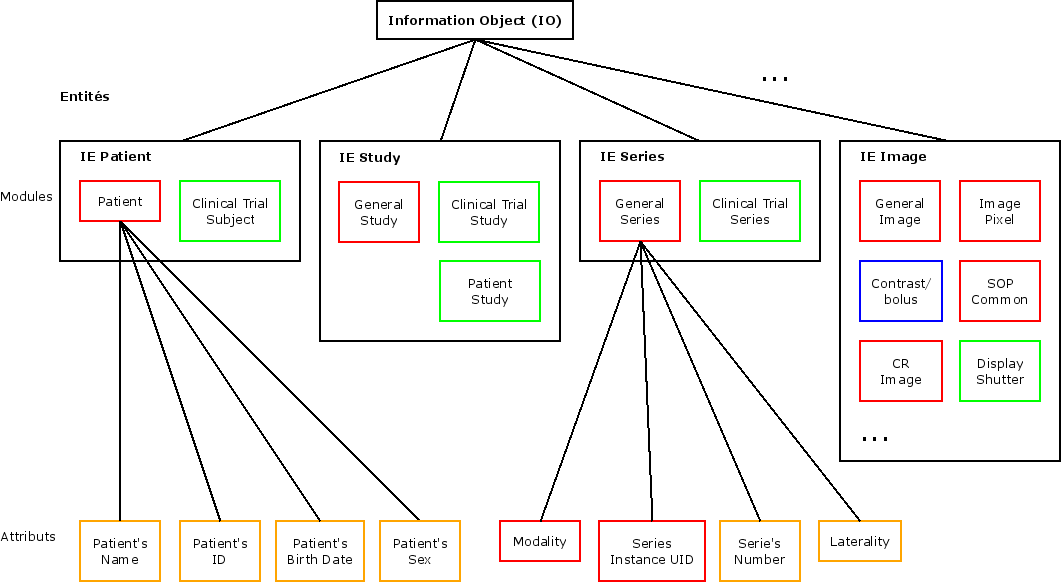
\includegraphics[width=\linewidth]{../figures/IO-definition.png}
		\end{center}
	}
	
    \frame
	{
		\frametitle{Syntaxe de transfert}
		\begin{itemize}
			\item Lorsque la modalit\'e souhaite stocker ses objets, elle doit s'assurer que le syst\`eme cible est capable de comprendre comment les donn\'ees sont repr\'esent\'ees.
			\item<2-> Se met alors en place une n\'egociation entre les deux sys\`emes:
			\begin{enumerate}
				\item<3-> La modalit\'e indique une liste de \emph{presentation contexts} (SOP avec une ou plusieurs syntaxes de tranfert) qu'elle est capable de fournir.
				\item<4-> L'archivage r\'epond en indiquant pour chaque \emph{presentation context} quelle syntaxe de transfert il accepte, ou s'il va tout refuser car il ne supporte aucune des syntaxes propos\'ees.
				\item<5-> La modalit\'e envoie les objets selon la syntaxe n\'egoci\'ee
			\end{enumerate}
			\item<6-> Par souci d'interop\'erabilit\'e, tout syst\^eme de stockage doit supporter au moins une syntaxe de transfert: \emph{Implicit~VR~Little~Endian}.
			\item<7-> Le mieux est \'evidemment quand l'archive peut stocker les objets dans leur format original.
			\item<8-> La liste des syntaxes de transfert se trouve dans le tableau 8.7.3{-}2 de la norme (\url{https://dicom.nema.org/medical/dicom/current/output/chtml/part18/sect_8.7.3.html}).
		\end{itemize}
	}

	\frame
	{
		\frametitle{Storage Commitment}
		\begin{itemize}
			\item Le but de ce service est de s'assurer que les \'el\'ements sont bien stock\'es.
			\item<2-> La modalit\'e fait une requ\^ete au syst\`eme d'archivage (PACS, VNA) avec la liste des UID des objets qui doivent avoir \'et\'e archiv\'es.
			\item<3-> La r\'eponse contient la liste des objets, et en cas d'\'echec, la cause de l'erreur (e.g. probl\`eme de ressources, objets non introuvables,\ldots).
			\item<4-> La modalit\'e peut repousser automatiquement tout objet non stock\'e.
			\item<5-> Peut se faire juste apr\`es le stockage ou de mani\`ere asynchrone (e.g. tous les jours \`a minuit).
			\item<6-> Limitation des risques, d\'emarche qualit\'e.
		\end{itemize}
	}
	
	\frame
	{
		\frametitle{Query/Retrieve}
		\begin{itemize}
			\item Une fois les objets sur l'archivage, d'autres syst\`emes peuvent vouloir y acc\'eder: stations de reconstruction, de navigation, d'interpr\^etation, autres PACS/VNA, etc.
			\item<2-> L'interrogation se fait par crit\`eres \`a diff\'erents niveaux (e.g. patient, examen, s\'erie, image, etc.).
			Ces crit\`eres peuvent se combiner, par exemple:
			\begin{itemize}
				\item<3-> tous les CT du jour,
				\item<4-> les examens des patients dont le nom commencent par DUP effectu\'es le mois dernier.
			\end{itemize}
			\item<5-> Les objets sont ensuite t\'el\'echarg\'es selon ces m\^emes crit\`eres.
		\end{itemize}
	}
    